\documentclass[border=3pt]{standalone}
\usepackage[T1]{fontenc}
\usepackage{lmodern}
\usepackage{amsmath,amssymb}
\usepackage{tikz}
\usepackage{pgfplots}
\pgfplotsset{compat=1.17}
\usepgfplotslibrary{groupplots}
\usetikzlibrary{arrows.meta,calc,positioning,fit,backgrounds}

% Industrial robotics: multi-camera tracking of parts for automated assembly.
\begin{document}
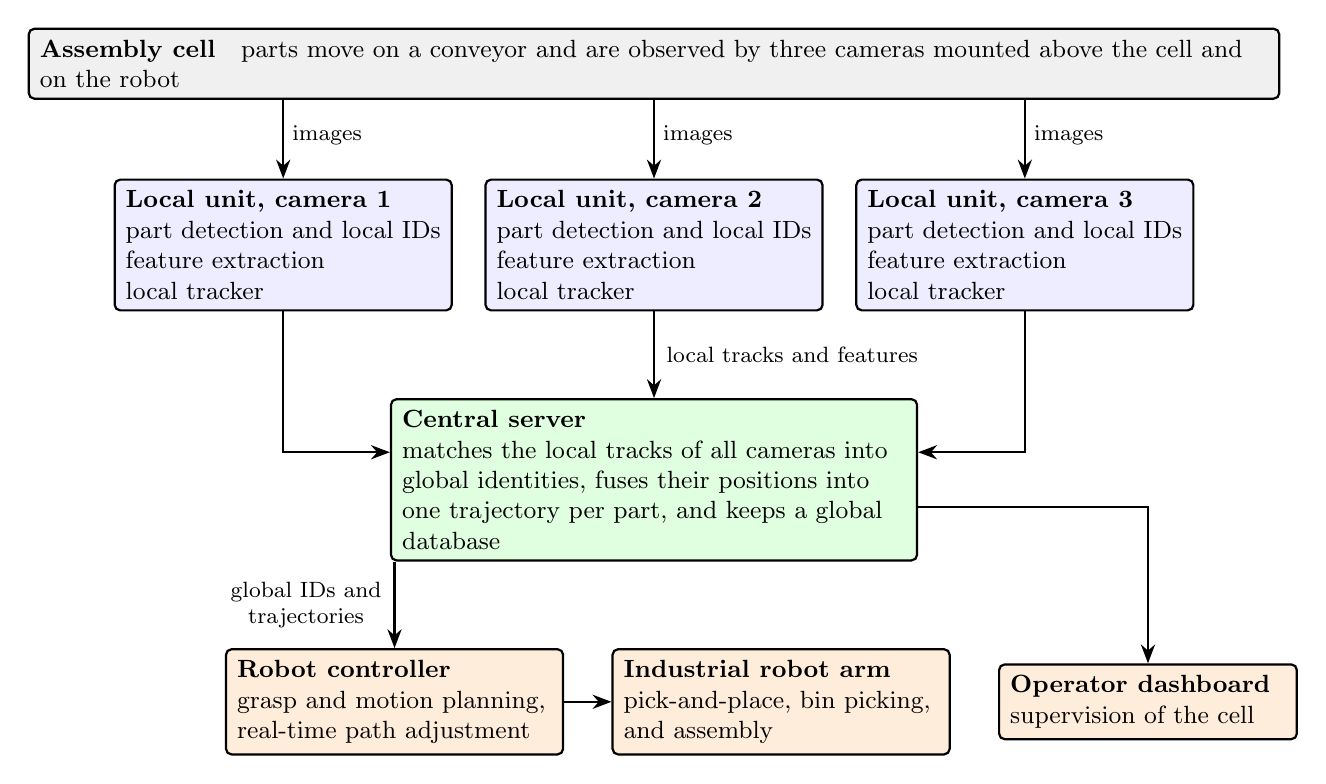
\begin{tikzpicture}[
  font=\small,
  sen/.style={draw, thick, rounded corners=2pt, fill=gray!12, align=flush left, text width=156mm, inner sep=4pt},
  loc/.style={draw, thick, rounded corners=2pt, fill=blue!7, align=flush left, text width=40mm, inner sep=4pt},
  srv/.style={draw, thick, rounded corners=2pt, fill=green!12, align=flush left, text width=64mm, inner sep=4pt},
  res/.style={draw, thick, rounded corners=2pt, fill=orange!14, align=flush left, text width=40mm, inner sep=4pt},
  arr/.style={-{Stealth[length=2.4mm]}, thick},
  lab/.style={font=\footnotesize, fill=white, inner sep=1.5pt, align=center}]
\node[sen] (cell) at (0,0) {\textbf{Assembly cell}\quad parts move on a conveyor and are observed by three
  cameras mounted above the cell and on the robot};
\node[loc, below=10mm of cell] (u2) {\textbf{Local unit, camera 2}\\ part detection and local IDs\\
  feature extraction\\ local tracker};
\node[loc, left=4mm of u2] (u1) {\textbf{Local unit, camera 1}\\ part detection and local IDs\\
  feature extraction\\ local tracker};
\node[loc, right=4mm of u2] (u3) {\textbf{Local unit, camera 3}\\ part detection and local IDs\\
  feature extraction\\ local tracker};
\node[srv, below=11mm of u2] (srv) {\textbf{Central server}\\ matches the local tracks of all cameras into
  global identities, fuses their positions into one trajectory per part, and keeps a global database};
\path (srv.south) ++(0,-11mm) coordinate (row);
\node[res, text width=40mm, anchor=north west] (ctl) at (row -| -5.45,0) {\textbf{Robot controller}\\
  grasp and motion planning, real-time path adjustment};
\node[res, text width=40mm, right=6mm of ctl] (arm) {\textbf{Industrial robot arm}\\ pick-and-place, bin picking, and assembly};
\node[res, text width=35mm, right=6mm of arm] (dash) {\textbf{Operator dashboard}\\ supervision of the cell};
\foreach \u in {u1,u2,u3} \draw[arr] (cell.south -| \u.north) -- node[lab, right=0.5mm, pos=0.45] {images} (\u.north);
\draw[arr] (u1.south) |- ($(srv.west)+(0,0.35)$);
\draw[arr] (u2.south) -- (srv.north);
\draw[arr] (u3.south) |- ($(srv.east)+(0,0.35)$);
\node[lab, anchor=west] at ($(u2.south)!0.5!(srv.north)+(0.1,0)$) {local tracks and features};
\draw[arr] (srv.south -| ctl.north) -- node[lab, left=1mm] {global IDs and\\ trajectories} (ctl.north);
\draw[arr] (ctl) -- (arm);
\draw[arr] ($(srv.east)+(0,-0.35)$) -| (dash.north);
\end{tikzpicture}
\end{document}
